\section{eo\-General\-Breeder$<$ EOT $>$ Class Template Reference}
\label{classeo_general_breeder}\index{eoGeneralBreeder@{eoGeneralBreeder}}
Base class for breeders using generalized operators.  


{\tt \#include $<$eo\-General\-Breeder.h$>$}

Inheritance diagram for eo\-General\-Breeder$<$ EOT $>$::\begin{figure}[H]
\begin{center}
\leavevmode
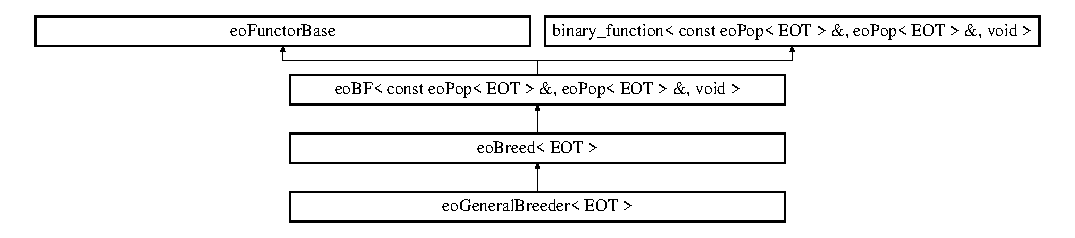
\includegraphics[height=2.75184cm]{classeo_general_breeder}
\end{center}
\end{figure}
\subsection*{Public Member Functions}
\begin{CompactItemize}
\item 
{\bf eo\-General\-Breeder} ({\bf eo\-Select\-One}$<$ {\bf EOT} $>$ \&\_\-select, {\bf eo\-Gen\-Op}$<$ {\bf EOT} $>$ \&\_\-op, double \_\-rate=1.0, bool \_\-interpret\_\-as\_\-rate=true)
\begin{CompactList}\small\item\em Ctor:. \item\end{CompactList}\item 
{\bf eo\-General\-Breeder} ({\bf eo\-Select\-One}$<$ {\bf EOT} $>$ \&\_\-select, {\bf eo\-Gen\-Op}$<$ {\bf EOT} $>$ \&\_\-op, {\bf eo\-How\-Many} \_\-how\-Many)
\begin{CompactList}\small\item\em Ctor:. \item\end{CompactList}\item 
void {\bf operator()} (const {\bf eo\-Pop}$<$ {\bf EOT} $>$ \&\_\-parents, {\bf eo\-Pop}$<$ {\bf EOT} $>$ \&\_\-offspring)
\begin{CompactList}\small\item\em The breeder: simply calls the gen\-Op on a selective populator! \item\end{CompactList}\item 
virtual std::string {\bf class\-Name} () const \label{classeo_general_breeder_a3}

\begin{CompactList}\small\item\em The class name. \item\end{CompactList}\end{CompactItemize}
\subsection*{Private Attributes}
\begin{CompactItemize}
\item 
{\bf eo\-Select\-One}$<$ {\bf EOT} $>$ \& {\bf select}\label{classeo_general_breeder_r0}

\item 
{\bf eo\-Gen\-Op}$<$ {\bf EOT} $>$ \& {\bf op}\label{classeo_general_breeder_r1}

\item 
{\bf eo\-How\-Many} {\bf how\-Many}\label{classeo_general_breeder_r2}

\end{CompactItemize}


\subsection{Detailed Description}
\subsubsection*{template$<$class EOT$>$ class eo\-General\-Breeder$<$ EOT $>$}

Base class for breeders using generalized operators. 



Definition at line 46 of file eo\-General\-Breeder.h.

\subsection{Constructor \& Destructor Documentation}
\index{eoGeneralBreeder@{eo\-General\-Breeder}!eoGeneralBreeder@{eoGeneralBreeder}}
\index{eoGeneralBreeder@{eoGeneralBreeder}!eoGeneralBreeder@{eo\-General\-Breeder}}
\subsubsection{\setlength{\rightskip}{0pt plus 5cm}template$<$class EOT$>$ {\bf eo\-General\-Breeder}$<$ {\bf EOT} $>$::{\bf eo\-General\-Breeder} ({\bf eo\-Select\-One}$<$ {\bf EOT} $>$ \& {\em \_\-select}, {\bf eo\-Gen\-Op}$<$ {\bf EOT} $>$ \& {\em \_\-op}, double {\em \_\-rate} = {\tt 1.0}, bool {\em \_\-interpret\_\-as\_\-rate} = {\tt true})\hspace{0.3cm}{\tt  [inline]}}\label{classeo_general_breeder_a0}


Ctor:. 

\begin{Desc}
\item[Parameters:]
\begin{description}
\item[{\em \_\-select}]a selecto\-One, to be used for all selections \item[{\em \_\-op}]a general operator (will generally be an {\bf eo\-Op\-Container}{\rm (p.\,\pageref{classeo_op_container})}) \item[{\em \_\-rate}]pour how\-Many, le nbre d'enfants a generer \item[{\em \_\-interpret\_\-as\_\-rate}]{\tt explanation} \end{description}
\end{Desc}


Definition at line 56 of file eo\-General\-Breeder.h.\index{eoGeneralBreeder@{eo\-General\-Breeder}!eoGeneralBreeder@{eoGeneralBreeder}}
\index{eoGeneralBreeder@{eoGeneralBreeder}!eoGeneralBreeder@{eo\-General\-Breeder}}
\subsubsection{\setlength{\rightskip}{0pt plus 5cm}template$<$class EOT$>$ {\bf eo\-General\-Breeder}$<$ {\bf EOT} $>$::{\bf eo\-General\-Breeder} ({\bf eo\-Select\-One}$<$ {\bf EOT} $>$ \& {\em \_\-select}, {\bf eo\-Gen\-Op}$<$ {\bf EOT} $>$ \& {\em \_\-op}, {\bf eo\-How\-Many} {\em \_\-how\-Many})\hspace{0.3cm}{\tt  [inline]}}\label{classeo_general_breeder_a1}


Ctor:. 

\begin{Desc}
\item[Parameters:]
\begin{description}
\item[{\em \_\-select}]a selecto\-One, to be used for all selections \item[{\em \_\-op}]a general operator (will generally be an {\bf eo\-Op\-Container}{\rm (p.\,\pageref{classeo_op_container})}) \item[{\em \_\-how\-Many}]an {\bf eo\-How\-Many}{\rm (p.\,\pageref{classeo_how_many})} {\tt explanation} \end{description}
\end{Desc}


Definition at line 69 of file eo\-General\-Breeder.h.

\subsection{Member Function Documentation}
\index{eoGeneralBreeder@{eo\-General\-Breeder}!operator()@{operator()}}
\index{operator()@{operator()}!eoGeneralBreeder@{eo\-General\-Breeder}}
\subsubsection{\setlength{\rightskip}{0pt plus 5cm}template$<$class EOT$>$ void {\bf eo\-General\-Breeder}$<$ {\bf EOT} $>$::operator() (const {\bf eo\-Pop}$<$ {\bf EOT} $>$ \& {\em \_\-parents}, {\bf eo\-Pop}$<$ {\bf EOT} $>$ \& {\em \_\-offspring})\hspace{0.3cm}{\tt  [inline, virtual]}}\label{classeo_general_breeder_a2}


The breeder: simply calls the gen\-Op on a selective populator! 

\begin{Desc}
\item[Parameters:]
\begin{description}
\item[{\em \_\-parents}]the initial population \item[{\em \_\-offspring}]the resulting population (content -if any- is lost) \end{description}
\end{Desc}


Implements {\bf eo\-BF$<$ const eo\-Pop$<$ EOT $>$ \&, eo\-Pop$<$ EOT $>$ \&, void $>$} {\rm (p.\,\pageref{classeo_b_f_a1})}.

Definition at line 80 of file eo\-General\-Breeder.h.

The documentation for this class was generated from the following file:\begin{CompactItemize}
\item 
eo\-General\-Breeder.h\end{CompactItemize}
